\documentclass[letterpaper,12pt]{article}
\usepackage[margin=0in]{geometry}
\usepackage[T1]{fontenc}
\usepackage{lmodern}
\pdfmapfile{+lm.map}
\pdfmapfile{+cm.map}
\usepackage{tikz}
\usetikzlibrary{arrows.meta}
\pagestyle{empty}
\setlength{\parindent}{0pt}
\hyphenpenalty=10000
\exhyphenpenalty=10000
\renewcommand{\familydefault}{\sfdefault}
\begin{document}
\begin{tikzpicture}[remember picture,overlay,x=1mm,y=1mm]
\begin{scope}[shift={(current page.north west)}]
\node[anchor=north west,inner sep=0pt,align=left,text width=180mm,font=\fontsize{11.5}{14}\selectfont\bfseries] at (18,-15.5) {Week 12 / Catalan bijections / Grades 2--3};
\node[anchor=north west,inner sep=0pt,align=left,text width=180mm,font=\fontsize{9}{11}\selectfont] at (18,-266.5) {Bellingham Math Circle / Week 12 / W12-23-v3};
\node[anchor=north east,inner sep=0pt,font=\fontsize{9}{11}\selectfont] at (198,-266.5) {1};
\node[anchor=north west,inner sep=0pt,align=left,text width=180mm,font=\fontsize{12.3}{15}\selectfont] at (18,-29) {Use each dot once. Keep strings above the row without crossings. Keep dots in place. Pairings are different when a dot has a different partner.};
\node[anchor=north west,inner sep=0pt,align=left,text width=180mm,font=\fontsize{12}{15}\selectfont] at (18,-50) {Example with ten dots:};
\draw[gray!45,line width=.35pt] (26,-77) -- (188,-77);
\draw[line width=.9pt] (26,-77) .. controls (26,-67.225) and (80,-67.225) .. (80,-77);
\draw[line width=.9pt] (44,-77) .. controls (44,-73.742) and (62,-73.742) .. (62,-77);
\draw[line width=.9pt] (98,-77) .. controls (98,-60.708) and (188,-60.708) .. (188,-77);
\draw[line width=.9pt] (116,-77) .. controls (116,-73.742) and (134,-73.742) .. (134,-77);
\draw[line width=.9pt] (152,-77) .. controls (152,-73.742) and (170,-73.742) .. (170,-77);
\fill (26,-77) circle (1.2mm);
\node[anchor=north,inner sep=0pt,font=\fontsize{9}{11}\selectfont] at (26,-79.4) {1};
\fill (44,-77) circle (1.2mm);
\node[anchor=north,inner sep=0pt,font=\fontsize{9}{11}\selectfont] at (44,-79.4) {2};
\fill (62,-77) circle (1.2mm);
\node[anchor=north,inner sep=0pt,font=\fontsize{9}{11}\selectfont] at (62,-79.4) {3};
\fill (80,-77) circle (1.2mm);
\node[anchor=north,inner sep=0pt,font=\fontsize{9}{11}\selectfont] at (80,-79.4) {4};
\fill (98,-77) circle (1.2mm);
\node[anchor=north,inner sep=0pt,font=\fontsize{9}{11}\selectfont] at (98,-79.4) {5};
\fill (116,-77) circle (1.2mm);
\node[anchor=north,inner sep=0pt,font=\fontsize{9}{11}\selectfont] at (116,-79.4) {6};
\fill (134,-77) circle (1.2mm);
\node[anchor=north,inner sep=0pt,font=\fontsize{9}{11}\selectfont] at (134,-79.4) {7};
\fill (152,-77) circle (1.2mm);
\node[anchor=north,inner sep=0pt,font=\fontsize{9}{11}\selectfont] at (152,-79.4) {8};
\fill (170,-77) circle (1.2mm);
\node[anchor=north,inner sep=0pt,font=\fontsize{9}{11}\selectfont] at (170,-79.4) {9};
\fill (188,-77) circle (1.2mm);
\node[anchor=north,inner sep=0pt,font=\fontsize{9}{11}\selectfont] at (188,-79.4) {10};
\node[anchor=north west,inner sep=0pt,align=left,text width=180mm,font=\fontsize{13}{16.5}\selectfont] at (18,-91) {\textbf{Problem 1:} Find every way to pair the six dots. Draw a complete collection with no repeats.};
\draw[gray!45,line width=.35pt] (48,-167) -- (168,-167);
\fill (48,-167) circle (1.6mm);
\node[anchor=north,inner sep=0pt,font=\fontsize{9}{11}\selectfont] at (48,-179.5) {1};
\fill (72,-167) circle (1.6mm);
\node[anchor=north,inner sep=0pt,font=\fontsize{9}{11}\selectfont] at (72,-179.5) {2};
\fill (96,-167) circle (1.6mm);
\node[anchor=north,inner sep=0pt,font=\fontsize{9}{11}\selectfont] at (96,-179.5) {3};
\fill (120,-167) circle (1.6mm);
\node[anchor=north,inner sep=0pt,font=\fontsize{9}{11}\selectfont] at (120,-179.5) {4};
\fill (144,-167) circle (1.6mm);
\node[anchor=north,inner sep=0pt,font=\fontsize{9}{11}\selectfont] at (144,-179.5) {5};
\fill (168,-167) circle (1.6mm);
\node[anchor=north,inner sep=0pt,font=\fontsize{9}{11}\selectfont] at (168,-179.5) {6};
\draw[gray!45,line width=.35pt] (25,-205) -- (85,-205);
\fill (25,-205) circle (1.2mm);
\node[anchor=north,inner sep=0pt,font=\fontsize{9}{11}\selectfont] at (25,-207.4) {1};
\fill (37,-205) circle (1.2mm);
\node[anchor=north,inner sep=0pt,font=\fontsize{9}{11}\selectfont] at (37,-207.4) {2};
\fill (49,-205) circle (1.2mm);
\node[anchor=north,inner sep=0pt,font=\fontsize{9}{11}\selectfont] at (49,-207.4) {3};
\fill (61,-205) circle (1.2mm);
\node[anchor=north,inner sep=0pt,font=\fontsize{9}{11}\selectfont] at (61,-207.4) {4};
\fill (73,-205) circle (1.2mm);
\node[anchor=north,inner sep=0pt,font=\fontsize{9}{11}\selectfont] at (73,-207.4) {5};
\fill (85,-205) circle (1.2mm);
\node[anchor=north,inner sep=0pt,font=\fontsize{9}{11}\selectfont] at (85,-207.4) {6};
\draw[gray!45,line width=.35pt] (123,-205) -- (183,-205);
\fill (123,-205) circle (1.2mm);
\node[anchor=north,inner sep=0pt,font=\fontsize{9}{11}\selectfont] at (123,-207.4) {1};
\fill (135,-205) circle (1.2mm);
\node[anchor=north,inner sep=0pt,font=\fontsize{9}{11}\selectfont] at (135,-207.4) {2};
\fill (147,-205) circle (1.2mm);
\node[anchor=north,inner sep=0pt,font=\fontsize{9}{11}\selectfont] at (147,-207.4) {3};
\fill (159,-205) circle (1.2mm);
\node[anchor=north,inner sep=0pt,font=\fontsize{9}{11}\selectfont] at (159,-207.4) {4};
\fill (171,-205) circle (1.2mm);
\node[anchor=north,inner sep=0pt,font=\fontsize{9}{11}\selectfont] at (171,-207.4) {5};
\fill (183,-205) circle (1.2mm);
\node[anchor=north,inner sep=0pt,font=\fontsize{9}{11}\selectfont] at (183,-207.4) {6};
\draw[gray!45,line width=.35pt] (25,-230) -- (85,-230);
\fill (25,-230) circle (1.2mm);
\node[anchor=north,inner sep=0pt,font=\fontsize{9}{11}\selectfont] at (25,-232.4) {1};
\fill (37,-230) circle (1.2mm);
\node[anchor=north,inner sep=0pt,font=\fontsize{9}{11}\selectfont] at (37,-232.4) {2};
\fill (49,-230) circle (1.2mm);
\node[anchor=north,inner sep=0pt,font=\fontsize{9}{11}\selectfont] at (49,-232.4) {3};
\fill (61,-230) circle (1.2mm);
\node[anchor=north,inner sep=0pt,font=\fontsize{9}{11}\selectfont] at (61,-232.4) {4};
\fill (73,-230) circle (1.2mm);
\node[anchor=north,inner sep=0pt,font=\fontsize{9}{11}\selectfont] at (73,-232.4) {5};
\fill (85,-230) circle (1.2mm);
\node[anchor=north,inner sep=0pt,font=\fontsize{9}{11}\selectfont] at (85,-232.4) {6};
\draw[gray!45,line width=.35pt] (123,-230) -- (183,-230);
\fill (123,-230) circle (1.2mm);
\node[anchor=north,inner sep=0pt,font=\fontsize{9}{11}\selectfont] at (123,-232.4) {1};
\fill (135,-230) circle (1.2mm);
\node[anchor=north,inner sep=0pt,font=\fontsize{9}{11}\selectfont] at (135,-232.4) {2};
\fill (147,-230) circle (1.2mm);
\node[anchor=north,inner sep=0pt,font=\fontsize{9}{11}\selectfont] at (147,-232.4) {3};
\fill (159,-230) circle (1.2mm);
\node[anchor=north,inner sep=0pt,font=\fontsize{9}{11}\selectfont] at (159,-232.4) {4};
\fill (171,-230) circle (1.2mm);
\node[anchor=north,inner sep=0pt,font=\fontsize{9}{11}\selectfont] at (171,-232.4) {5};
\fill (183,-230) circle (1.2mm);
\node[anchor=north,inner sep=0pt,font=\fontsize{9}{11}\selectfont] at (183,-232.4) {6};
\draw[gray!45,line width=.35pt] (25,-255) -- (85,-255);
\fill (25,-255) circle (1.2mm);
\node[anchor=north,inner sep=0pt,font=\fontsize{9}{11}\selectfont] at (25,-257.4) {1};
\fill (37,-255) circle (1.2mm);
\node[anchor=north,inner sep=0pt,font=\fontsize{9}{11}\selectfont] at (37,-257.4) {2};
\fill (49,-255) circle (1.2mm);
\node[anchor=north,inner sep=0pt,font=\fontsize{9}{11}\selectfont] at (49,-257.4) {3};
\fill (61,-255) circle (1.2mm);
\node[anchor=north,inner sep=0pt,font=\fontsize{9}{11}\selectfont] at (61,-257.4) {4};
\fill (73,-255) circle (1.2mm);
\node[anchor=north,inner sep=0pt,font=\fontsize{9}{11}\selectfont] at (73,-257.4) {5};
\fill (85,-255) circle (1.2mm);
\node[anchor=north,inner sep=0pt,font=\fontsize{9}{11}\selectfont] at (85,-257.4) {6};
\draw[gray!45,line width=.35pt] (123,-255) -- (183,-255);
\fill (123,-255) circle (1.2mm);
\node[anchor=north,inner sep=0pt,font=\fontsize{9}{11}\selectfont] at (123,-257.4) {1};
\fill (135,-255) circle (1.2mm);
\node[anchor=north,inner sep=0pt,font=\fontsize{9}{11}\selectfont] at (135,-257.4) {2};
\fill (147,-255) circle (1.2mm);
\node[anchor=north,inner sep=0pt,font=\fontsize{9}{11}\selectfont] at (147,-257.4) {3};
\fill (159,-255) circle (1.2mm);
\node[anchor=north,inner sep=0pt,font=\fontsize{9}{11}\selectfont] at (159,-257.4) {4};
\fill (171,-255) circle (1.2mm);
\node[anchor=north,inner sep=0pt,font=\fontsize{9}{11}\selectfont] at (171,-257.4) {5};
\fill (183,-255) circle (1.2mm);
\node[anchor=north,inner sep=0pt,font=\fontsize{9}{11}\selectfont] at (183,-257.4) {6};
\end{scope}
\end{tikzpicture}
\null
\newpage
\begin{tikzpicture}[remember picture,overlay,x=1mm,y=1mm]
\begin{scope}[shift={(current page.north west)}]
\node[anchor=north west,inner sep=0pt,align=left,text width=180mm,font=\fontsize{11.5}{14}\selectfont\bfseries] at (18,-15.5) {Week 12 / Catalan bijections / Grades 2--3};
\node[anchor=north west,inner sep=0pt,align=left,text width=180mm,font=\fontsize{9}{11}\selectfont] at (18,-266.5) {Bellingham Math Circle / Week 12 / W12-23-v3};
\node[anchor=north east,inner sep=0pt,font=\fontsize{9}{11}\selectfont] at (198,-266.5) {2};
\node[anchor=north west,inner sep=0pt,align=left,text width=180mm,font=\fontsize{12.3}{15.5}\selectfont] at (18,-29) {Read the dots from left to right. Write U at the first end of each pair and D at the other end. U is one step up and right; D is one step down and right.};
\node[anchor=north west,inner sep=0pt,align=left,text width=180mm,font=\fontsize{12}{15}\selectfont] at (18,-56) {Example:};
\draw[gray!45,line width=.35pt] (25,-91) -- (96.4,-91);
\draw[line width=.9pt] (25,-91) .. controls (25,-86.62) and (35.2,-86.62) .. (35.2,-91);
\draw[line width=.9pt] (45.4,-91) .. controls (45.4,-77.86) and (76,-77.86) .. (76,-91);
\draw[line width=.9pt] (55.6,-91) .. controls (55.6,-86.62) and (65.8,-86.62) .. (65.8,-91);
\draw[line width=.9pt] (86.2,-91) .. controls (86.2,-86.62) and (96.4,-86.62) .. (96.4,-91);
\fill (25,-91) circle (1.2mm);
\node[anchor=north,inner sep=0pt,font=\fontsize{9}{11}\selectfont] at (25,-93.4) {1};
\fill (35.2,-91) circle (1.2mm);
\node[anchor=north,inner sep=0pt,font=\fontsize{9}{11}\selectfont] at (35.2,-93.4) {2};
\fill (45.4,-91) circle (1.2mm);
\node[anchor=north,inner sep=0pt,font=\fontsize{9}{11}\selectfont] at (45.4,-93.4) {3};
\fill (55.6,-91) circle (1.2mm);
\node[anchor=north,inner sep=0pt,font=\fontsize{9}{11}\selectfont] at (55.6,-93.4) {4};
\fill (65.8,-91) circle (1.2mm);
\node[anchor=north,inner sep=0pt,font=\fontsize{9}{11}\selectfont] at (65.8,-93.4) {5};
\fill (76,-91) circle (1.2mm);
\node[anchor=north,inner sep=0pt,font=\fontsize{9}{11}\selectfont] at (76,-93.4) {6};
\fill (86.2,-91) circle (1.2mm);
\node[anchor=north,inner sep=0pt,font=\fontsize{9}{11}\selectfont] at (86.2,-93.4) {7};
\fill (96.4,-91) circle (1.2mm);
\node[anchor=north,inner sep=0pt,font=\fontsize{9}{11}\selectfont] at (96.4,-93.4) {8};
\node[anchor=north west,inner sep=0pt,align=left,text width=6mm,font=\fontsize{12}{14}\selectfont] at (23.5,-102) {U};
\node[anchor=north west,inner sep=0pt,align=left,text width=6mm,font=\fontsize{12}{14}\selectfont] at (33.7,-102) {D};
\node[anchor=north west,inner sep=0pt,align=left,text width=6mm,font=\fontsize{12}{14}\selectfont] at (43.9,-102) {U};
\node[anchor=north west,inner sep=0pt,align=left,text width=6mm,font=\fontsize{12}{14}\selectfont] at (54.1,-102) {U};
\node[anchor=north west,inner sep=0pt,align=left,text width=6mm,font=\fontsize{12}{14}\selectfont] at (64.3,-102) {D};
\node[anchor=north west,inner sep=0pt,align=left,text width=6mm,font=\fontsize{12}{14}\selectfont] at (74.5,-102) {D};
\node[anchor=north west,inner sep=0pt,align=left,text width=6mm,font=\fontsize{12}{14}\selectfont] at (84.7,-102) {U};
\node[anchor=north west,inner sep=0pt,align=left,text width=6mm,font=\fontsize{12}{14}\selectfont] at (94.9,-102) {D};
\draw[gray!35,line width=.25pt] (126,-103) -- (126,-79);
\draw[gray!35,line width=.25pt] (134,-103) -- (134,-79);
\draw[gray!35,line width=.25pt] (142,-103) -- (142,-79);
\draw[gray!35,line width=.25pt] (150,-103) -- (150,-79);
\draw[gray!35,line width=.25pt] (158,-103) -- (158,-79);
\draw[gray!35,line width=.25pt] (166,-103) -- (166,-79);
\draw[gray!35,line width=.25pt] (174,-103) -- (174,-79);
\draw[gray!35,line width=.25pt] (182,-103) -- (182,-79);
\draw[gray!35,line width=.25pt] (190,-103) -- (190,-79);
\draw[gray!35,line width=.25pt] (126,-103) -- (190,-103);
\draw[gray!35,line width=.25pt] (126,-95) -- (190,-95);
\draw[gray!35,line width=.25pt] (126,-87) -- (190,-87);
\draw[gray!35,line width=.25pt] (126,-79) -- (190,-79);
\draw[line width=.8pt] (126,-103) -- (190,-103);
\draw[line width=1.15pt,line join=round] (126,-103) -- (134,-95) -- (142,-103) -- (150,-95) -- (158,-87) -- (166,-95) -- (174,-103) -- (182,-95) -- (190,-103);
\node[anchor=north west,inner sep=0pt,align=left,text width=5mm,font=\fontsize{9}{10}\selectfont] at (128.8,-94) {U};
\node[anchor=north west,inner sep=0pt,align=left,text width=5mm,font=\fontsize{9}{10}\selectfont] at (136.8,-94) {D};
\node[anchor=north west,inner sep=0pt,align=left,text width=5mm,font=\fontsize{9}{10}\selectfont] at (144.8,-94) {U};
\node[anchor=north west,inner sep=0pt,align=left,text width=5mm,font=\fontsize{9}{10}\selectfont] at (152.8,-86) {U};
\node[anchor=north west,inner sep=0pt,align=left,text width=5mm,font=\fontsize{9}{10}\selectfont] at (160.8,-86) {D};
\node[anchor=north west,inner sep=0pt,align=left,text width=5mm,font=\fontsize{9}{10}\selectfont] at (168.8,-94) {D};
\node[anchor=north west,inner sep=0pt,align=left,text width=5mm,font=\fontsize{9}{10}\selectfont] at (176.8,-94) {U};
\node[anchor=north west,inner sep=0pt,align=left,text width=5mm,font=\fontsize{9}{10}\selectfont] at (184.8,-94) {D};
\fill (126,-103) circle (1.3mm);
\draw[fill=white,line width=.8pt] (190,-103) circle (1.3mm);
\node[anchor=north west,inner sep=0pt,align=left,text width=180mm,font=\fontsize{13}{16.5}\selectfont] at (18,-120) {\textbf{Problem 2:} Draw the path for each pairing, starting at the marked dot. How does the height of each path compare with its starting level?};
\draw[gray!45,line width=.35pt] (25,-167) -- (85,-167);
\draw[line width=.9pt] (25,-167) .. controls (25,-136.341) and (85,-136.341) .. (85,-167);
\draw[line width=.9pt] (37,-167) .. controls (37,-148.605) and (73,-148.605) .. (73,-167);
\draw[line width=.9pt] (49,-167) .. controls (49,-160.868) and (61,-160.868) .. (61,-167);
\fill (25,-167) circle (1.2mm);
\node[anchor=north,inner sep=0pt,font=\fontsize{9}{11}\selectfont] at (25,-169.4) {1};
\fill (37,-167) circle (1.2mm);
\node[anchor=north,inner sep=0pt,font=\fontsize{9}{11}\selectfont] at (37,-169.4) {2};
\fill (49,-167) circle (1.2mm);
\node[anchor=north,inner sep=0pt,font=\fontsize{9}{11}\selectfont] at (49,-169.4) {3};
\fill (61,-167) circle (1.2mm);
\node[anchor=north,inner sep=0pt,font=\fontsize{9}{11}\selectfont] at (61,-169.4) {4};
\fill (73,-167) circle (1.2mm);
\node[anchor=north,inner sep=0pt,font=\fontsize{9}{11}\selectfont] at (73,-169.4) {5};
\fill (85,-167) circle (1.2mm);
\node[anchor=north,inner sep=0pt,font=\fontsize{9}{11}\selectfont] at (85,-169.4) {6};
\draw[gray!65,line width=.45pt] (34,-176) rectangle (41,-183);
\draw[gray!65,line width=.45pt] (41,-176) rectangle (48,-183);
\draw[gray!65,line width=.45pt] (48,-176) rectangle (55,-183);
\draw[gray!65,line width=.45pt] (55,-176) rectangle (62,-183);
\draw[gray!65,line width=.45pt] (62,-176) rectangle (69,-183);
\draw[gray!65,line width=.45pt] (69,-176) rectangle (76,-183);
\draw[gray!35,line width=.25pt] (126,-170) -- (126,-146);
\draw[gray!35,line width=.25pt] (134,-170) -- (134,-146);
\draw[gray!35,line width=.25pt] (142,-170) -- (142,-146);
\draw[gray!35,line width=.25pt] (150,-170) -- (150,-146);
\draw[gray!35,line width=.25pt] (158,-170) -- (158,-146);
\draw[gray!35,line width=.25pt] (166,-170) -- (166,-146);
\draw[gray!35,line width=.25pt] (174,-170) -- (174,-146);
\draw[gray!35,line width=.25pt] (126,-170) -- (174,-170);
\draw[gray!35,line width=.25pt] (126,-162) -- (174,-162);
\draw[gray!35,line width=.25pt] (126,-154) -- (174,-154);
\draw[gray!35,line width=.25pt] (126,-146) -- (174,-146);
\draw[line width=.8pt] (126,-170) -- (174,-170);
\fill (126,-170) circle (1.3mm);
\draw[fill=white,line width=.8pt] (174,-170) circle (1.3mm);
\draw[gray!45,line width=.35pt] (25,-207) -- (85,-207);
\draw[line width=.9pt] (25,-207) .. controls (25,-188.605) and (61,-188.605) .. (61,-207);
\draw[line width=.9pt] (37,-207) .. controls (37,-200.868) and (49,-200.868) .. (49,-207);
\draw[line width=.9pt] (73,-207) .. controls (73,-200.868) and (85,-200.868) .. (85,-207);
\fill (25,-207) circle (1.2mm);
\node[anchor=north,inner sep=0pt,font=\fontsize{9}{11}\selectfont] at (25,-209.4) {1};
\fill (37,-207) circle (1.2mm);
\node[anchor=north,inner sep=0pt,font=\fontsize{9}{11}\selectfont] at (37,-209.4) {2};
\fill (49,-207) circle (1.2mm);
\node[anchor=north,inner sep=0pt,font=\fontsize{9}{11}\selectfont] at (49,-209.4) {3};
\fill (61,-207) circle (1.2mm);
\node[anchor=north,inner sep=0pt,font=\fontsize{9}{11}\selectfont] at (61,-209.4) {4};
\fill (73,-207) circle (1.2mm);
\node[anchor=north,inner sep=0pt,font=\fontsize{9}{11}\selectfont] at (73,-209.4) {5};
\fill (85,-207) circle (1.2mm);
\node[anchor=north,inner sep=0pt,font=\fontsize{9}{11}\selectfont] at (85,-209.4) {6};
\draw[gray!65,line width=.45pt] (34,-216) rectangle (41,-223);
\draw[gray!65,line width=.45pt] (41,-216) rectangle (48,-223);
\draw[gray!65,line width=.45pt] (48,-216) rectangle (55,-223);
\draw[gray!65,line width=.45pt] (55,-216) rectangle (62,-223);
\draw[gray!65,line width=.45pt] (62,-216) rectangle (69,-223);
\draw[gray!65,line width=.45pt] (69,-216) rectangle (76,-223);
\draw[gray!35,line width=.25pt] (126,-210) -- (126,-186);
\draw[gray!35,line width=.25pt] (134,-210) -- (134,-186);
\draw[gray!35,line width=.25pt] (142,-210) -- (142,-186);
\draw[gray!35,line width=.25pt] (150,-210) -- (150,-186);
\draw[gray!35,line width=.25pt] (158,-210) -- (158,-186);
\draw[gray!35,line width=.25pt] (166,-210) -- (166,-186);
\draw[gray!35,line width=.25pt] (174,-210) -- (174,-186);
\draw[gray!35,line width=.25pt] (126,-210) -- (174,-210);
\draw[gray!35,line width=.25pt] (126,-202) -- (174,-202);
\draw[gray!35,line width=.25pt] (126,-194) -- (174,-194);
\draw[gray!35,line width=.25pt] (126,-186) -- (174,-186);
\draw[line width=.8pt] (126,-210) -- (174,-210);
\fill (126,-210) circle (1.3mm);
\draw[fill=white,line width=.8pt] (174,-210) circle (1.3mm);
\draw[gray!45,line width=.35pt] (25,-247) -- (85,-247);
\draw[line width=.9pt] (25,-247) .. controls (25,-240.868) and (37,-240.868) .. (37,-247);
\draw[line width=.9pt] (49,-247) .. controls (49,-240.868) and (61,-240.868) .. (61,-247);
\draw[line width=.9pt] (73,-247) .. controls (73,-240.868) and (85,-240.868) .. (85,-247);
\fill (25,-247) circle (1.2mm);
\node[anchor=north,inner sep=0pt,font=\fontsize{9}{11}\selectfont] at (25,-249.4) {1};
\fill (37,-247) circle (1.2mm);
\node[anchor=north,inner sep=0pt,font=\fontsize{9}{11}\selectfont] at (37,-249.4) {2};
\fill (49,-247) circle (1.2mm);
\node[anchor=north,inner sep=0pt,font=\fontsize{9}{11}\selectfont] at (49,-249.4) {3};
\fill (61,-247) circle (1.2mm);
\node[anchor=north,inner sep=0pt,font=\fontsize{9}{11}\selectfont] at (61,-249.4) {4};
\fill (73,-247) circle (1.2mm);
\node[anchor=north,inner sep=0pt,font=\fontsize{9}{11}\selectfont] at (73,-249.4) {5};
\fill (85,-247) circle (1.2mm);
\node[anchor=north,inner sep=0pt,font=\fontsize{9}{11}\selectfont] at (85,-249.4) {6};
\draw[gray!65,line width=.45pt] (34,-256) rectangle (41,-263);
\draw[gray!65,line width=.45pt] (41,-256) rectangle (48,-263);
\draw[gray!65,line width=.45pt] (48,-256) rectangle (55,-263);
\draw[gray!65,line width=.45pt] (55,-256) rectangle (62,-263);
\draw[gray!65,line width=.45pt] (62,-256) rectangle (69,-263);
\draw[gray!65,line width=.45pt] (69,-256) rectangle (76,-263);
\draw[gray!35,line width=.25pt] (126,-250) -- (126,-226);
\draw[gray!35,line width=.25pt] (134,-250) -- (134,-226);
\draw[gray!35,line width=.25pt] (142,-250) -- (142,-226);
\draw[gray!35,line width=.25pt] (150,-250) -- (150,-226);
\draw[gray!35,line width=.25pt] (158,-250) -- (158,-226);
\draw[gray!35,line width=.25pt] (166,-250) -- (166,-226);
\draw[gray!35,line width=.25pt] (174,-250) -- (174,-226);
\draw[gray!35,line width=.25pt] (126,-250) -- (174,-250);
\draw[gray!35,line width=.25pt] (126,-242) -- (174,-242);
\draw[gray!35,line width=.25pt] (126,-234) -- (174,-234);
\draw[gray!35,line width=.25pt] (126,-226) -- (174,-226);
\draw[line width=.8pt] (126,-250) -- (174,-250);
\fill (126,-250) circle (1.3mm);
\draw[fill=white,line width=.8pt] (174,-250) circle (1.3mm);
\end{scope}
\end{tikzpicture}
\null
\newpage
\begin{tikzpicture}[remember picture,overlay,x=1mm,y=1mm]
\begin{scope}[shift={(current page.north west)}]
\node[anchor=north west,inner sep=0pt,align=left,text width=180mm,font=\fontsize{11.5}{14}\selectfont\bfseries] at (18,-15.5) {Week 12 / Catalan bijections / Grades 2--3};
\node[anchor=north west,inner sep=0pt,align=left,text width=180mm,font=\fontsize{9}{11}\selectfont] at (18,-266.5) {Bellingham Math Circle / Week 12 / W12-23-v3};
\node[anchor=north east,inner sep=0pt,font=\fontsize{9}{11}\selectfont] at (198,-266.5) {3};
\node[anchor=north west,inner sep=0pt,align=left,text width=180mm,font=\fontsize{13}{16.5}\selectfont] at (18,-30) {\textbf{Problem 3:} Draw a pairing for each path. Could a path come from two different pairings without crossings? Explain.};
\draw[gray!35,line width=.25pt] (23,-91) -- (23,-68.5);
\draw[gray!35,line width=.25pt] (30.5,-91) -- (30.5,-68.5);
\draw[gray!35,line width=.25pt] (38,-91) -- (38,-68.5);
\draw[gray!35,line width=.25pt] (45.5,-91) -- (45.5,-68.5);
\draw[gray!35,line width=.25pt] (53,-91) -- (53,-68.5);
\draw[gray!35,line width=.25pt] (60.5,-91) -- (60.5,-68.5);
\draw[gray!35,line width=.25pt] (68,-91) -- (68,-68.5);
\draw[gray!35,line width=.25pt] (23,-91) -- (68,-91);
\draw[gray!35,line width=.25pt] (23,-83.5) -- (68,-83.5);
\draw[gray!35,line width=.25pt] (23,-76) -- (68,-76);
\draw[gray!35,line width=.25pt] (23,-68.5) -- (68,-68.5);
\draw[line width=.8pt] (23,-91) -- (68,-91);
\draw[line width=1.15pt,line join=round] (23,-91) -- (30.5,-83.5) -- (38,-76) -- (45.5,-83.5) -- (53,-76) -- (60.5,-83.5) -- (68,-91);
\fill (23,-91) circle (1.3mm);
\draw[fill=white,line width=.8pt] (68,-91) circle (1.3mm);
\draw[gray!45,line width=.35pt] (119,-91) -- (170.5,-91);
\fill (119,-91) circle (1.2mm);
\node[anchor=north,inner sep=0pt,font=\fontsize{9}{11}\selectfont] at (119,-93.4) {1};
\fill (129.3,-91) circle (1.2mm);
\node[anchor=north,inner sep=0pt,font=\fontsize{9}{11}\selectfont] at (129.3,-93.4) {2};
\fill (139.6,-91) circle (1.2mm);
\node[anchor=north,inner sep=0pt,font=\fontsize{9}{11}\selectfont] at (139.6,-93.4) {3};
\fill (149.9,-91) circle (1.2mm);
\node[anchor=north,inner sep=0pt,font=\fontsize{9}{11}\selectfont] at (149.9,-93.4) {4};
\fill (160.2,-91) circle (1.2mm);
\node[anchor=north,inner sep=0pt,font=\fontsize{9}{11}\selectfont] at (160.2,-93.4) {5};
\fill (170.5,-91) circle (1.2mm);
\node[anchor=north,inner sep=0pt,font=\fontsize{9}{11}\selectfont] at (170.5,-93.4) {6};
\draw[gray!35,line width=.25pt] (23,-143) -- (23,-120.5);
\draw[gray!35,line width=.25pt] (30.5,-143) -- (30.5,-120.5);
\draw[gray!35,line width=.25pt] (38,-143) -- (38,-120.5);
\draw[gray!35,line width=.25pt] (45.5,-143) -- (45.5,-120.5);
\draw[gray!35,line width=.25pt] (53,-143) -- (53,-120.5);
\draw[gray!35,line width=.25pt] (60.5,-143) -- (60.5,-120.5);
\draw[gray!35,line width=.25pt] (68,-143) -- (68,-120.5);
\draw[gray!35,line width=.25pt] (23,-143) -- (68,-143);
\draw[gray!35,line width=.25pt] (23,-135.5) -- (68,-135.5);
\draw[gray!35,line width=.25pt] (23,-128) -- (68,-128);
\draw[gray!35,line width=.25pt] (23,-120.5) -- (68,-120.5);
\draw[line width=.8pt] (23,-143) -- (68,-143);
\draw[line width=1.15pt,line join=round] (23,-143) -- (30.5,-135.5) -- (38,-143) -- (45.5,-135.5) -- (53,-128) -- (60.5,-135.5) -- (68,-143);
\fill (23,-143) circle (1.3mm);
\draw[fill=white,line width=.8pt] (68,-143) circle (1.3mm);
\draw[gray!45,line width=.35pt] (119,-143) -- (170.5,-143);
\fill (119,-143) circle (1.2mm);
\node[anchor=north,inner sep=0pt,font=\fontsize{9}{11}\selectfont] at (119,-145.4) {1};
\fill (129.3,-143) circle (1.2mm);
\node[anchor=north,inner sep=0pt,font=\fontsize{9}{11}\selectfont] at (129.3,-145.4) {2};
\fill (139.6,-143) circle (1.2mm);
\node[anchor=north,inner sep=0pt,font=\fontsize{9}{11}\selectfont] at (139.6,-145.4) {3};
\fill (149.9,-143) circle (1.2mm);
\node[anchor=north,inner sep=0pt,font=\fontsize{9}{11}\selectfont] at (149.9,-145.4) {4};
\fill (160.2,-143) circle (1.2mm);
\node[anchor=north,inner sep=0pt,font=\fontsize{9}{11}\selectfont] at (160.2,-145.4) {5};
\fill (170.5,-143) circle (1.2mm);
\node[anchor=north,inner sep=0pt,font=\fontsize{9}{11}\selectfont] at (170.5,-145.4) {6};
\draw[gray!35,line width=.25pt] (23,-195) -- (23,-165);
\draw[gray!35,line width=.25pt] (30.5,-195) -- (30.5,-165);
\draw[gray!35,line width=.25pt] (38,-195) -- (38,-165);
\draw[gray!35,line width=.25pt] (45.5,-195) -- (45.5,-165);
\draw[gray!35,line width=.25pt] (53,-195) -- (53,-165);
\draw[gray!35,line width=.25pt] (60.5,-195) -- (60.5,-165);
\draw[gray!35,line width=.25pt] (68,-195) -- (68,-165);
\draw[gray!35,line width=.25pt] (75.5,-195) -- (75.5,-165);
\draw[gray!35,line width=.25pt] (83,-195) -- (83,-165);
\draw[gray!35,line width=.25pt] (23,-195) -- (83,-195);
\draw[gray!35,line width=.25pt] (23,-187.5) -- (83,-187.5);
\draw[gray!35,line width=.25pt] (23,-180) -- (83,-180);
\draw[gray!35,line width=.25pt] (23,-172.5) -- (83,-172.5);
\draw[gray!35,line width=.25pt] (23,-165) -- (83,-165);
\draw[line width=.8pt] (23,-195) -- (83,-195);
\draw[line width=1.15pt,line join=round] (23,-195) -- (30.5,-187.5) -- (38,-180) -- (45.5,-187.5) -- (53,-195) -- (60.5,-187.5) -- (68,-180) -- (75.5,-187.5) -- (83,-195);
\fill (23,-195) circle (1.3mm);
\draw[fill=white,line width=.8pt] (83,-195) circle (1.3mm);
\draw[gray!45,line width=.35pt] (119,-195) -- (191.1,-195);
\fill (119,-195) circle (1.2mm);
\node[anchor=north,inner sep=0pt,font=\fontsize{9}{11}\selectfont] at (119,-197.4) {1};
\fill (129.3,-195) circle (1.2mm);
\node[anchor=north,inner sep=0pt,font=\fontsize{9}{11}\selectfont] at (129.3,-197.4) {2};
\fill (139.6,-195) circle (1.2mm);
\node[anchor=north,inner sep=0pt,font=\fontsize{9}{11}\selectfont] at (139.6,-197.4) {3};
\fill (149.9,-195) circle (1.2mm);
\node[anchor=north,inner sep=0pt,font=\fontsize{9}{11}\selectfont] at (149.9,-197.4) {4};
\fill (160.2,-195) circle (1.2mm);
\node[anchor=north,inner sep=0pt,font=\fontsize{9}{11}\selectfont] at (160.2,-197.4) {5};
\fill (170.5,-195) circle (1.2mm);
\node[anchor=north,inner sep=0pt,font=\fontsize{9}{11}\selectfont] at (170.5,-197.4) {6};
\fill (180.8,-195) circle (1.2mm);
\node[anchor=north,inner sep=0pt,font=\fontsize{9}{11}\selectfont] at (180.8,-197.4) {7};
\fill (191.1,-195) circle (1.2mm);
\node[anchor=north,inner sep=0pt,font=\fontsize{9}{11}\selectfont] at (191.1,-197.4) {8};
\draw[gray!35,line width=.25pt] (23,-247) -- (23,-217);
\draw[gray!35,line width=.25pt] (30.5,-247) -- (30.5,-217);
\draw[gray!35,line width=.25pt] (38,-247) -- (38,-217);
\draw[gray!35,line width=.25pt] (45.5,-247) -- (45.5,-217);
\draw[gray!35,line width=.25pt] (53,-247) -- (53,-217);
\draw[gray!35,line width=.25pt] (60.5,-247) -- (60.5,-217);
\draw[gray!35,line width=.25pt] (68,-247) -- (68,-217);
\draw[gray!35,line width=.25pt] (75.5,-247) -- (75.5,-217);
\draw[gray!35,line width=.25pt] (83,-247) -- (83,-217);
\draw[gray!35,line width=.25pt] (23,-247) -- (83,-247);
\draw[gray!35,line width=.25pt] (23,-239.5) -- (83,-239.5);
\draw[gray!35,line width=.25pt] (23,-232) -- (83,-232);
\draw[gray!35,line width=.25pt] (23,-224.5) -- (83,-224.5);
\draw[gray!35,line width=.25pt] (23,-217) -- (83,-217);
\draw[line width=.8pt] (23,-247) -- (83,-247);
\draw[line width=1.15pt,line join=round] (23,-247) -- (30.5,-239.5) -- (38,-232) -- (45.5,-224.5) -- (53,-232) -- (60.5,-224.5) -- (68,-232) -- (75.5,-239.5) -- (83,-247);
\fill (23,-247) circle (1.3mm);
\draw[fill=white,line width=.8pt] (83,-247) circle (1.3mm);
\draw[gray!45,line width=.35pt] (119,-247) -- (191.1,-247);
\fill (119,-247) circle (1.2mm);
\node[anchor=north,inner sep=0pt,font=\fontsize{9}{11}\selectfont] at (119,-249.4) {1};
\fill (129.3,-247) circle (1.2mm);
\node[anchor=north,inner sep=0pt,font=\fontsize{9}{11}\selectfont] at (129.3,-249.4) {2};
\fill (139.6,-247) circle (1.2mm);
\node[anchor=north,inner sep=0pt,font=\fontsize{9}{11}\selectfont] at (139.6,-249.4) {3};
\fill (149.9,-247) circle (1.2mm);
\node[anchor=north,inner sep=0pt,font=\fontsize{9}{11}\selectfont] at (149.9,-249.4) {4};
\fill (160.2,-247) circle (1.2mm);
\node[anchor=north,inner sep=0pt,font=\fontsize{9}{11}\selectfont] at (160.2,-249.4) {5};
\fill (170.5,-247) circle (1.2mm);
\node[anchor=north,inner sep=0pt,font=\fontsize{9}{11}\selectfont] at (170.5,-249.4) {6};
\fill (180.8,-247) circle (1.2mm);
\node[anchor=north,inner sep=0pt,font=\fontsize{9}{11}\selectfont] at (180.8,-249.4) {7};
\fill (191.1,-247) circle (1.2mm);
\node[anchor=north,inner sep=0pt,font=\fontsize{9}{11}\selectfont] at (191.1,-249.4) {8};
\end{scope}
\end{tikzpicture}
\null
\newpage
\begin{tikzpicture}[remember picture,overlay,x=1mm,y=1mm]
\begin{scope}[shift={(current page.north west)}]
\node[anchor=north west,inner sep=0pt,align=left,text width=180mm,font=\fontsize{11.5}{14}\selectfont\bfseries] at (18,-15.5) {Week 12 / Catalan bijections / Grades 2--3};
\node[anchor=north west,inner sep=0pt,align=left,text width=180mm,font=\fontsize{9}{11}\selectfont] at (18,-266.5) {Bellingham Math Circle / Week 12 / W12-23-v3};
\node[anchor=north east,inner sep=0pt,font=\fontsize{9}{11}\selectfont] at (198,-266.5) {4};
\node[anchor=north west,inner sep=0pt,align=left,text width=180mm,font=\fontsize{13}{16.5}\selectfont] at (18,-30) {\textbf{Problem 4:} Find every path with three up steps and three down steps that starts and ends on the dark line and never goes below it. Match your paths to your six-dot pairings.};
\draw[gray!35,line width=.25pt] (27,-105) -- (27,-75);
\draw[gray!35,line width=.25pt] (37,-105) -- (37,-75);
\draw[gray!35,line width=.25pt] (47,-105) -- (47,-75);
\draw[gray!35,line width=.25pt] (57,-105) -- (57,-75);
\draw[gray!35,line width=.25pt] (67,-105) -- (67,-75);
\draw[gray!35,line width=.25pt] (77,-105) -- (77,-75);
\draw[gray!35,line width=.25pt] (87,-105) -- (87,-75);
\draw[gray!35,line width=.25pt] (27,-105) -- (87,-105);
\draw[gray!35,line width=.25pt] (27,-95) -- (87,-95);
\draw[gray!35,line width=.25pt] (27,-85) -- (87,-85);
\draw[gray!35,line width=.25pt] (27,-75) -- (87,-75);
\draw[line width=.8pt] (27,-105) -- (87,-105);
\fill (27,-105) circle (1.3mm);
\draw[fill=white,line width=.8pt] (87,-105) circle (1.3mm);
\draw[gray!35,line width=.25pt] (126,-105) -- (126,-75);
\draw[gray!35,line width=.25pt] (136,-105) -- (136,-75);
\draw[gray!35,line width=.25pt] (146,-105) -- (146,-75);
\draw[gray!35,line width=.25pt] (156,-105) -- (156,-75);
\draw[gray!35,line width=.25pt] (166,-105) -- (166,-75);
\draw[gray!35,line width=.25pt] (176,-105) -- (176,-75);
\draw[gray!35,line width=.25pt] (186,-105) -- (186,-75);
\draw[gray!35,line width=.25pt] (126,-105) -- (186,-105);
\draw[gray!35,line width=.25pt] (126,-95) -- (186,-95);
\draw[gray!35,line width=.25pt] (126,-85) -- (186,-85);
\draw[gray!35,line width=.25pt] (126,-75) -- (186,-75);
\draw[line width=.8pt] (126,-105) -- (186,-105);
\fill (126,-105) circle (1.3mm);
\draw[fill=white,line width=.8pt] (186,-105) circle (1.3mm);
\draw[gray!35,line width=.25pt] (27,-167) -- (27,-137);
\draw[gray!35,line width=.25pt] (37,-167) -- (37,-137);
\draw[gray!35,line width=.25pt] (47,-167) -- (47,-137);
\draw[gray!35,line width=.25pt] (57,-167) -- (57,-137);
\draw[gray!35,line width=.25pt] (67,-167) -- (67,-137);
\draw[gray!35,line width=.25pt] (77,-167) -- (77,-137);
\draw[gray!35,line width=.25pt] (87,-167) -- (87,-137);
\draw[gray!35,line width=.25pt] (27,-167) -- (87,-167);
\draw[gray!35,line width=.25pt] (27,-157) -- (87,-157);
\draw[gray!35,line width=.25pt] (27,-147) -- (87,-147);
\draw[gray!35,line width=.25pt] (27,-137) -- (87,-137);
\draw[line width=.8pt] (27,-167) -- (87,-167);
\fill (27,-167) circle (1.3mm);
\draw[fill=white,line width=.8pt] (87,-167) circle (1.3mm);
\draw[gray!35,line width=.25pt] (126,-167) -- (126,-137);
\draw[gray!35,line width=.25pt] (136,-167) -- (136,-137);
\draw[gray!35,line width=.25pt] (146,-167) -- (146,-137);
\draw[gray!35,line width=.25pt] (156,-167) -- (156,-137);
\draw[gray!35,line width=.25pt] (166,-167) -- (166,-137);
\draw[gray!35,line width=.25pt] (176,-167) -- (176,-137);
\draw[gray!35,line width=.25pt] (186,-167) -- (186,-137);
\draw[gray!35,line width=.25pt] (126,-167) -- (186,-167);
\draw[gray!35,line width=.25pt] (126,-157) -- (186,-157);
\draw[gray!35,line width=.25pt] (126,-147) -- (186,-147);
\draw[gray!35,line width=.25pt] (126,-137) -- (186,-137);
\draw[line width=.8pt] (126,-167) -- (186,-167);
\fill (126,-167) circle (1.3mm);
\draw[fill=white,line width=.8pt] (186,-167) circle (1.3mm);
\draw[gray!35,line width=.25pt] (27,-229) -- (27,-199);
\draw[gray!35,line width=.25pt] (37,-229) -- (37,-199);
\draw[gray!35,line width=.25pt] (47,-229) -- (47,-199);
\draw[gray!35,line width=.25pt] (57,-229) -- (57,-199);
\draw[gray!35,line width=.25pt] (67,-229) -- (67,-199);
\draw[gray!35,line width=.25pt] (77,-229) -- (77,-199);
\draw[gray!35,line width=.25pt] (87,-229) -- (87,-199);
\draw[gray!35,line width=.25pt] (27,-229) -- (87,-229);
\draw[gray!35,line width=.25pt] (27,-219) -- (87,-219);
\draw[gray!35,line width=.25pt] (27,-209) -- (87,-209);
\draw[gray!35,line width=.25pt] (27,-199) -- (87,-199);
\draw[line width=.8pt] (27,-229) -- (87,-229);
\fill (27,-229) circle (1.3mm);
\draw[fill=white,line width=.8pt] (87,-229) circle (1.3mm);
\draw[gray!35,line width=.25pt] (126,-229) -- (126,-199);
\draw[gray!35,line width=.25pt] (136,-229) -- (136,-199);
\draw[gray!35,line width=.25pt] (146,-229) -- (146,-199);
\draw[gray!35,line width=.25pt] (156,-229) -- (156,-199);
\draw[gray!35,line width=.25pt] (166,-229) -- (166,-199);
\draw[gray!35,line width=.25pt] (176,-229) -- (176,-199);
\draw[gray!35,line width=.25pt] (186,-229) -- (186,-199);
\draw[gray!35,line width=.25pt] (126,-229) -- (186,-229);
\draw[gray!35,line width=.25pt] (126,-219) -- (186,-219);
\draw[gray!35,line width=.25pt] (126,-209) -- (186,-209);
\draw[gray!35,line width=.25pt] (126,-199) -- (186,-199);
\draw[line width=.8pt] (126,-229) -- (186,-229);
\fill (126,-229) circle (1.3mm);
\draw[fill=white,line width=.8pt] (186,-229) circle (1.3mm);
\end{scope}
\end{tikzpicture}
\null
\newpage
\begin{tikzpicture}[remember picture,overlay,x=1mm,y=1mm]
\begin{scope}[shift={(current page.north west)}]
\node[anchor=north west,inner sep=0pt,align=left,text width=180mm,font=\fontsize{11.5}{14}\selectfont\bfseries] at (18,-15.5) {Week 12 / Catalan bijections / Grades 2--3};
\node[anchor=north west,inner sep=0pt,align=left,text width=180mm,font=\fontsize{9}{11}\selectfont] at (18,-266.5) {Bellingham Math Circle / Week 12 / W12-23-v3};
\node[anchor=north east,inner sep=0pt,font=\fontsize{9}{11}\selectfont] at (198,-266.5) {5};
\node[anchor=north west,inner sep=0pt,align=left,text width=180mm,font=\fontsize{13}{16.5}\selectfont] at (18,-30) {\textbf{Problem 5:} Which strings of letters can be codes for pairings of eight dots? Draw the pairing whenever it is possible, and explain what goes wrong whenever it is impossible.};
\node[anchor=north west,inner sep=0pt,align=left,text width=82mm,font=\fontsize{15}{18}\selectfont] at (21,-74) {\texttt{UUUDDUDD}};
\draw[gray!45,line width=.35pt] (109,-101) -- (188.8,-101);
\fill (109,-101) circle (1.2mm);
\node[anchor=north,inner sep=0pt,font=\fontsize{9}{11}\selectfont] at (109,-103.4) {1};
\fill (120.4,-101) circle (1.2mm);
\node[anchor=north,inner sep=0pt,font=\fontsize{9}{11}\selectfont] at (120.4,-103.4) {2};
\fill (131.8,-101) circle (1.2mm);
\node[anchor=north,inner sep=0pt,font=\fontsize{9}{11}\selectfont] at (131.8,-103.4) {3};
\fill (143.2,-101) circle (1.2mm);
\node[anchor=north,inner sep=0pt,font=\fontsize{9}{11}\selectfont] at (143.2,-103.4) {4};
\fill (154.6,-101) circle (1.2mm);
\node[anchor=north,inner sep=0pt,font=\fontsize{9}{11}\selectfont] at (154.6,-103.4) {5};
\fill (166,-101) circle (1.2mm);
\node[anchor=north,inner sep=0pt,font=\fontsize{9}{11}\selectfont] at (166,-103.4) {6};
\fill (177.4,-101) circle (1.2mm);
\node[anchor=north,inner sep=0pt,font=\fontsize{9}{11}\selectfont] at (177.4,-103.4) {7};
\fill (188.8,-101) circle (1.2mm);
\node[anchor=north,inner sep=0pt,font=\fontsize{9}{11}\selectfont] at (188.8,-103.4) {8};
\node[anchor=north west,inner sep=0pt,align=left,text width=82mm,font=\fontsize{15}{18}\selectfont] at (21,-122) {\texttt{UDDUUDUD}};
\draw[gray!45,line width=.35pt] (109,-149) -- (188.8,-149);
\fill (109,-149) circle (1.2mm);
\node[anchor=north,inner sep=0pt,font=\fontsize{9}{11}\selectfont] at (109,-151.4) {1};
\fill (120.4,-149) circle (1.2mm);
\node[anchor=north,inner sep=0pt,font=\fontsize{9}{11}\selectfont] at (120.4,-151.4) {2};
\fill (131.8,-149) circle (1.2mm);
\node[anchor=north,inner sep=0pt,font=\fontsize{9}{11}\selectfont] at (131.8,-151.4) {3};
\fill (143.2,-149) circle (1.2mm);
\node[anchor=north,inner sep=0pt,font=\fontsize{9}{11}\selectfont] at (143.2,-151.4) {4};
\fill (154.6,-149) circle (1.2mm);
\node[anchor=north,inner sep=0pt,font=\fontsize{9}{11}\selectfont] at (154.6,-151.4) {5};
\fill (166,-149) circle (1.2mm);
\node[anchor=north,inner sep=0pt,font=\fontsize{9}{11}\selectfont] at (166,-151.4) {6};
\fill (177.4,-149) circle (1.2mm);
\node[anchor=north,inner sep=0pt,font=\fontsize{9}{11}\selectfont] at (177.4,-151.4) {7};
\fill (188.8,-149) circle (1.2mm);
\node[anchor=north,inner sep=0pt,font=\fontsize{9}{11}\selectfont] at (188.8,-151.4) {8};
\node[anchor=north west,inner sep=0pt,align=left,text width=82mm,font=\fontsize{15}{18}\selectfont] at (21,-170) {\texttt{UUDUDUDD}};
\draw[gray!45,line width=.35pt] (109,-197) -- (188.8,-197);
\fill (109,-197) circle (1.2mm);
\node[anchor=north,inner sep=0pt,font=\fontsize{9}{11}\selectfont] at (109,-199.4) {1};
\fill (120.4,-197) circle (1.2mm);
\node[anchor=north,inner sep=0pt,font=\fontsize{9}{11}\selectfont] at (120.4,-199.4) {2};
\fill (131.8,-197) circle (1.2mm);
\node[anchor=north,inner sep=0pt,font=\fontsize{9}{11}\selectfont] at (131.8,-199.4) {3};
\fill (143.2,-197) circle (1.2mm);
\node[anchor=north,inner sep=0pt,font=\fontsize{9}{11}\selectfont] at (143.2,-199.4) {4};
\fill (154.6,-197) circle (1.2mm);
\node[anchor=north,inner sep=0pt,font=\fontsize{9}{11}\selectfont] at (154.6,-199.4) {5};
\fill (166,-197) circle (1.2mm);
\node[anchor=north,inner sep=0pt,font=\fontsize{9}{11}\selectfont] at (166,-199.4) {6};
\fill (177.4,-197) circle (1.2mm);
\node[anchor=north,inner sep=0pt,font=\fontsize{9}{11}\selectfont] at (177.4,-199.4) {7};
\fill (188.8,-197) circle (1.2mm);
\node[anchor=north,inner sep=0pt,font=\fontsize{9}{11}\selectfont] at (188.8,-199.4) {8};
\node[anchor=north west,inner sep=0pt,align=left,text width=82mm,font=\fontsize{15}{18}\selectfont] at (21,-218) {\texttt{UUUUDDUD}};
\draw[gray!45,line width=.35pt] (109,-245) -- (188.8,-245);
\fill (109,-245) circle (1.2mm);
\node[anchor=north,inner sep=0pt,font=\fontsize{9}{11}\selectfont] at (109,-247.4) {1};
\fill (120.4,-245) circle (1.2mm);
\node[anchor=north,inner sep=0pt,font=\fontsize{9}{11}\selectfont] at (120.4,-247.4) {2};
\fill (131.8,-245) circle (1.2mm);
\node[anchor=north,inner sep=0pt,font=\fontsize{9}{11}\selectfont] at (131.8,-247.4) {3};
\fill (143.2,-245) circle (1.2mm);
\node[anchor=north,inner sep=0pt,font=\fontsize{9}{11}\selectfont] at (143.2,-247.4) {4};
\fill (154.6,-245) circle (1.2mm);
\node[anchor=north,inner sep=0pt,font=\fontsize{9}{11}\selectfont] at (154.6,-247.4) {5};
\fill (166,-245) circle (1.2mm);
\node[anchor=north,inner sep=0pt,font=\fontsize{9}{11}\selectfont] at (166,-247.4) {6};
\fill (177.4,-245) circle (1.2mm);
\node[anchor=north,inner sep=0pt,font=\fontsize{9}{11}\selectfont] at (177.4,-247.4) {7};
\fill (188.8,-245) circle (1.2mm);
\node[anchor=north,inner sep=0pt,font=\fontsize{9}{11}\selectfont] at (188.8,-247.4) {8};
\end{scope}
\end{tikzpicture}
\null
\newpage
\begin{tikzpicture}[remember picture,overlay,x=1mm,y=1mm]
\begin{scope}[shift={(current page.north west)}]
\node[anchor=north west,inner sep=0pt,align=left,text width=180mm,font=\fontsize{11.5}{14}\selectfont\bfseries] at (18,-15.5) {Week 12 / Catalan bijections / Grades 2--3};
\node[anchor=north west,inner sep=0pt,align=left,text width=180mm,font=\fontsize{9}{11}\selectfont] at (18,-266.5) {Bellingham Math Circle / Week 12 / W12-23-v3};
\node[anchor=north east,inner sep=0pt,font=\fontsize{9}{11}\selectfont] at (198,-266.5) {6};
\node[anchor=north west,inner sep=0pt,align=left,text width=180mm,font=\fontsize{13}{16.5}\selectfont] at (18,-30) {\textbf{Problem 6:} Draw every pairing of eight dots. How can you be sure that none are missing?};
\draw[gray!45,line width=.35pt] (23,-70) -- (96.5,-70);
\fill (23,-70) circle (1.05mm);
\node[anchor=north,inner sep=0pt,font=\fontsize{9}{11}\selectfont] at (23,-72.4) {1};
\fill (33.5,-70) circle (1.05mm);
\node[anchor=north,inner sep=0pt,font=\fontsize{9}{11}\selectfont] at (33.5,-72.4) {2};
\fill (44,-70) circle (1.05mm);
\node[anchor=north,inner sep=0pt,font=\fontsize{9}{11}\selectfont] at (44,-72.4) {3};
\fill (54.5,-70) circle (1.05mm);
\node[anchor=north,inner sep=0pt,font=\fontsize{9}{11}\selectfont] at (54.5,-72.4) {4};
\fill (65,-70) circle (1.05mm);
\node[anchor=north,inner sep=0pt,font=\fontsize{9}{11}\selectfont] at (65,-72.4) {5};
\fill (75.5,-70) circle (1.05mm);
\node[anchor=north,inner sep=0pt,font=\fontsize{9}{11}\selectfont] at (75.5,-72.4) {6};
\fill (86,-70) circle (1.05mm);
\node[anchor=north,inner sep=0pt,font=\fontsize{9}{11}\selectfont] at (86,-72.4) {7};
\fill (96.5,-70) circle (1.05mm);
\node[anchor=north,inner sep=0pt,font=\fontsize{9}{11}\selectfont] at (96.5,-72.4) {8};
\draw[gray!45,line width=.35pt] (121,-70) -- (194.5,-70);
\fill (121,-70) circle (1.05mm);
\node[anchor=north,inner sep=0pt,font=\fontsize{9}{11}\selectfont] at (121,-72.4) {1};
\fill (131.5,-70) circle (1.05mm);
\node[anchor=north,inner sep=0pt,font=\fontsize{9}{11}\selectfont] at (131.5,-72.4) {2};
\fill (142,-70) circle (1.05mm);
\node[anchor=north,inner sep=0pt,font=\fontsize{9}{11}\selectfont] at (142,-72.4) {3};
\fill (152.5,-70) circle (1.05mm);
\node[anchor=north,inner sep=0pt,font=\fontsize{9}{11}\selectfont] at (152.5,-72.4) {4};
\fill (163,-70) circle (1.05mm);
\node[anchor=north,inner sep=0pt,font=\fontsize{9}{11}\selectfont] at (163,-72.4) {5};
\fill (173.5,-70) circle (1.05mm);
\node[anchor=north,inner sep=0pt,font=\fontsize{9}{11}\selectfont] at (173.5,-72.4) {6};
\fill (184,-70) circle (1.05mm);
\node[anchor=north,inner sep=0pt,font=\fontsize{9}{11}\selectfont] at (184,-72.4) {7};
\fill (194.5,-70) circle (1.05mm);
\node[anchor=north,inner sep=0pt,font=\fontsize{9}{11}\selectfont] at (194.5,-72.4) {8};
\draw[gray!45,line width=.35pt] (23,-96) -- (96.5,-96);
\fill (23,-96) circle (1.05mm);
\node[anchor=north,inner sep=0pt,font=\fontsize{9}{11}\selectfont] at (23,-98.4) {1};
\fill (33.5,-96) circle (1.05mm);
\node[anchor=north,inner sep=0pt,font=\fontsize{9}{11}\selectfont] at (33.5,-98.4) {2};
\fill (44,-96) circle (1.05mm);
\node[anchor=north,inner sep=0pt,font=\fontsize{9}{11}\selectfont] at (44,-98.4) {3};
\fill (54.5,-96) circle (1.05mm);
\node[anchor=north,inner sep=0pt,font=\fontsize{9}{11}\selectfont] at (54.5,-98.4) {4};
\fill (65,-96) circle (1.05mm);
\node[anchor=north,inner sep=0pt,font=\fontsize{9}{11}\selectfont] at (65,-98.4) {5};
\fill (75.5,-96) circle (1.05mm);
\node[anchor=north,inner sep=0pt,font=\fontsize{9}{11}\selectfont] at (75.5,-98.4) {6};
\fill (86,-96) circle (1.05mm);
\node[anchor=north,inner sep=0pt,font=\fontsize{9}{11}\selectfont] at (86,-98.4) {7};
\fill (96.5,-96) circle (1.05mm);
\node[anchor=north,inner sep=0pt,font=\fontsize{9}{11}\selectfont] at (96.5,-98.4) {8};
\draw[gray!45,line width=.35pt] (121,-96) -- (194.5,-96);
\fill (121,-96) circle (1.05mm);
\node[anchor=north,inner sep=0pt,font=\fontsize{9}{11}\selectfont] at (121,-98.4) {1};
\fill (131.5,-96) circle (1.05mm);
\node[anchor=north,inner sep=0pt,font=\fontsize{9}{11}\selectfont] at (131.5,-98.4) {2};
\fill (142,-96) circle (1.05mm);
\node[anchor=north,inner sep=0pt,font=\fontsize{9}{11}\selectfont] at (142,-98.4) {3};
\fill (152.5,-96) circle (1.05mm);
\node[anchor=north,inner sep=0pt,font=\fontsize{9}{11}\selectfont] at (152.5,-98.4) {4};
\fill (163,-96) circle (1.05mm);
\node[anchor=north,inner sep=0pt,font=\fontsize{9}{11}\selectfont] at (163,-98.4) {5};
\fill (173.5,-96) circle (1.05mm);
\node[anchor=north,inner sep=0pt,font=\fontsize{9}{11}\selectfont] at (173.5,-98.4) {6};
\fill (184,-96) circle (1.05mm);
\node[anchor=north,inner sep=0pt,font=\fontsize{9}{11}\selectfont] at (184,-98.4) {7};
\fill (194.5,-96) circle (1.05mm);
\node[anchor=north,inner sep=0pt,font=\fontsize{9}{11}\selectfont] at (194.5,-98.4) {8};
\draw[gray!45,line width=.35pt] (23,-122) -- (96.5,-122);
\fill (23,-122) circle (1.05mm);
\node[anchor=north,inner sep=0pt,font=\fontsize{9}{11}\selectfont] at (23,-124.4) {1};
\fill (33.5,-122) circle (1.05mm);
\node[anchor=north,inner sep=0pt,font=\fontsize{9}{11}\selectfont] at (33.5,-124.4) {2};
\fill (44,-122) circle (1.05mm);
\node[anchor=north,inner sep=0pt,font=\fontsize{9}{11}\selectfont] at (44,-124.4) {3};
\fill (54.5,-122) circle (1.05mm);
\node[anchor=north,inner sep=0pt,font=\fontsize{9}{11}\selectfont] at (54.5,-124.4) {4};
\fill (65,-122) circle (1.05mm);
\node[anchor=north,inner sep=0pt,font=\fontsize{9}{11}\selectfont] at (65,-124.4) {5};
\fill (75.5,-122) circle (1.05mm);
\node[anchor=north,inner sep=0pt,font=\fontsize{9}{11}\selectfont] at (75.5,-124.4) {6};
\fill (86,-122) circle (1.05mm);
\node[anchor=north,inner sep=0pt,font=\fontsize{9}{11}\selectfont] at (86,-124.4) {7};
\fill (96.5,-122) circle (1.05mm);
\node[anchor=north,inner sep=0pt,font=\fontsize{9}{11}\selectfont] at (96.5,-124.4) {8};
\draw[gray!45,line width=.35pt] (121,-122) -- (194.5,-122);
\fill (121,-122) circle (1.05mm);
\node[anchor=north,inner sep=0pt,font=\fontsize{9}{11}\selectfont] at (121,-124.4) {1};
\fill (131.5,-122) circle (1.05mm);
\node[anchor=north,inner sep=0pt,font=\fontsize{9}{11}\selectfont] at (131.5,-124.4) {2};
\fill (142,-122) circle (1.05mm);
\node[anchor=north,inner sep=0pt,font=\fontsize{9}{11}\selectfont] at (142,-124.4) {3};
\fill (152.5,-122) circle (1.05mm);
\node[anchor=north,inner sep=0pt,font=\fontsize{9}{11}\selectfont] at (152.5,-124.4) {4};
\fill (163,-122) circle (1.05mm);
\node[anchor=north,inner sep=0pt,font=\fontsize{9}{11}\selectfont] at (163,-124.4) {5};
\fill (173.5,-122) circle (1.05mm);
\node[anchor=north,inner sep=0pt,font=\fontsize{9}{11}\selectfont] at (173.5,-124.4) {6};
\fill (184,-122) circle (1.05mm);
\node[anchor=north,inner sep=0pt,font=\fontsize{9}{11}\selectfont] at (184,-124.4) {7};
\fill (194.5,-122) circle (1.05mm);
\node[anchor=north,inner sep=0pt,font=\fontsize{9}{11}\selectfont] at (194.5,-124.4) {8};
\draw[gray!45,line width=.35pt] (23,-148) -- (96.5,-148);
\fill (23,-148) circle (1.05mm);
\node[anchor=north,inner sep=0pt,font=\fontsize{9}{11}\selectfont] at (23,-150.4) {1};
\fill (33.5,-148) circle (1.05mm);
\node[anchor=north,inner sep=0pt,font=\fontsize{9}{11}\selectfont] at (33.5,-150.4) {2};
\fill (44,-148) circle (1.05mm);
\node[anchor=north,inner sep=0pt,font=\fontsize{9}{11}\selectfont] at (44,-150.4) {3};
\fill (54.5,-148) circle (1.05mm);
\node[anchor=north,inner sep=0pt,font=\fontsize{9}{11}\selectfont] at (54.5,-150.4) {4};
\fill (65,-148) circle (1.05mm);
\node[anchor=north,inner sep=0pt,font=\fontsize{9}{11}\selectfont] at (65,-150.4) {5};
\fill (75.5,-148) circle (1.05mm);
\node[anchor=north,inner sep=0pt,font=\fontsize{9}{11}\selectfont] at (75.5,-150.4) {6};
\fill (86,-148) circle (1.05mm);
\node[anchor=north,inner sep=0pt,font=\fontsize{9}{11}\selectfont] at (86,-150.4) {7};
\fill (96.5,-148) circle (1.05mm);
\node[anchor=north,inner sep=0pt,font=\fontsize{9}{11}\selectfont] at (96.5,-150.4) {8};
\draw[gray!45,line width=.35pt] (121,-148) -- (194.5,-148);
\fill (121,-148) circle (1.05mm);
\node[anchor=north,inner sep=0pt,font=\fontsize{9}{11}\selectfont] at (121,-150.4) {1};
\fill (131.5,-148) circle (1.05mm);
\node[anchor=north,inner sep=0pt,font=\fontsize{9}{11}\selectfont] at (131.5,-150.4) {2};
\fill (142,-148) circle (1.05mm);
\node[anchor=north,inner sep=0pt,font=\fontsize{9}{11}\selectfont] at (142,-150.4) {3};
\fill (152.5,-148) circle (1.05mm);
\node[anchor=north,inner sep=0pt,font=\fontsize{9}{11}\selectfont] at (152.5,-150.4) {4};
\fill (163,-148) circle (1.05mm);
\node[anchor=north,inner sep=0pt,font=\fontsize{9}{11}\selectfont] at (163,-150.4) {5};
\fill (173.5,-148) circle (1.05mm);
\node[anchor=north,inner sep=0pt,font=\fontsize{9}{11}\selectfont] at (173.5,-150.4) {6};
\fill (184,-148) circle (1.05mm);
\node[anchor=north,inner sep=0pt,font=\fontsize{9}{11}\selectfont] at (184,-150.4) {7};
\fill (194.5,-148) circle (1.05mm);
\node[anchor=north,inner sep=0pt,font=\fontsize{9}{11}\selectfont] at (194.5,-150.4) {8};
\draw[gray!45,line width=.35pt] (23,-174) -- (96.5,-174);
\fill (23,-174) circle (1.05mm);
\node[anchor=north,inner sep=0pt,font=\fontsize{9}{11}\selectfont] at (23,-176.4) {1};
\fill (33.5,-174) circle (1.05mm);
\node[anchor=north,inner sep=0pt,font=\fontsize{9}{11}\selectfont] at (33.5,-176.4) {2};
\fill (44,-174) circle (1.05mm);
\node[anchor=north,inner sep=0pt,font=\fontsize{9}{11}\selectfont] at (44,-176.4) {3};
\fill (54.5,-174) circle (1.05mm);
\node[anchor=north,inner sep=0pt,font=\fontsize{9}{11}\selectfont] at (54.5,-176.4) {4};
\fill (65,-174) circle (1.05mm);
\node[anchor=north,inner sep=0pt,font=\fontsize{9}{11}\selectfont] at (65,-176.4) {5};
\fill (75.5,-174) circle (1.05mm);
\node[anchor=north,inner sep=0pt,font=\fontsize{9}{11}\selectfont] at (75.5,-176.4) {6};
\fill (86,-174) circle (1.05mm);
\node[anchor=north,inner sep=0pt,font=\fontsize{9}{11}\selectfont] at (86,-176.4) {7};
\fill (96.5,-174) circle (1.05mm);
\node[anchor=north,inner sep=0pt,font=\fontsize{9}{11}\selectfont] at (96.5,-176.4) {8};
\draw[gray!45,line width=.35pt] (121,-174) -- (194.5,-174);
\fill (121,-174) circle (1.05mm);
\node[anchor=north,inner sep=0pt,font=\fontsize{9}{11}\selectfont] at (121,-176.4) {1};
\fill (131.5,-174) circle (1.05mm);
\node[anchor=north,inner sep=0pt,font=\fontsize{9}{11}\selectfont] at (131.5,-176.4) {2};
\fill (142,-174) circle (1.05mm);
\node[anchor=north,inner sep=0pt,font=\fontsize{9}{11}\selectfont] at (142,-176.4) {3};
\fill (152.5,-174) circle (1.05mm);
\node[anchor=north,inner sep=0pt,font=\fontsize{9}{11}\selectfont] at (152.5,-176.4) {4};
\fill (163,-174) circle (1.05mm);
\node[anchor=north,inner sep=0pt,font=\fontsize{9}{11}\selectfont] at (163,-176.4) {5};
\fill (173.5,-174) circle (1.05mm);
\node[anchor=north,inner sep=0pt,font=\fontsize{9}{11}\selectfont] at (173.5,-176.4) {6};
\fill (184,-174) circle (1.05mm);
\node[anchor=north,inner sep=0pt,font=\fontsize{9}{11}\selectfont] at (184,-176.4) {7};
\fill (194.5,-174) circle (1.05mm);
\node[anchor=north,inner sep=0pt,font=\fontsize{9}{11}\selectfont] at (194.5,-176.4) {8};
\draw[gray!45,line width=.35pt] (23,-200) -- (96.5,-200);
\fill (23,-200) circle (1.05mm);
\node[anchor=north,inner sep=0pt,font=\fontsize{9}{11}\selectfont] at (23,-202.4) {1};
\fill (33.5,-200) circle (1.05mm);
\node[anchor=north,inner sep=0pt,font=\fontsize{9}{11}\selectfont] at (33.5,-202.4) {2};
\fill (44,-200) circle (1.05mm);
\node[anchor=north,inner sep=0pt,font=\fontsize{9}{11}\selectfont] at (44,-202.4) {3};
\fill (54.5,-200) circle (1.05mm);
\node[anchor=north,inner sep=0pt,font=\fontsize{9}{11}\selectfont] at (54.5,-202.4) {4};
\fill (65,-200) circle (1.05mm);
\node[anchor=north,inner sep=0pt,font=\fontsize{9}{11}\selectfont] at (65,-202.4) {5};
\fill (75.5,-200) circle (1.05mm);
\node[anchor=north,inner sep=0pt,font=\fontsize{9}{11}\selectfont] at (75.5,-202.4) {6};
\fill (86,-200) circle (1.05mm);
\node[anchor=north,inner sep=0pt,font=\fontsize{9}{11}\selectfont] at (86,-202.4) {7};
\fill (96.5,-200) circle (1.05mm);
\node[anchor=north,inner sep=0pt,font=\fontsize{9}{11}\selectfont] at (96.5,-202.4) {8};
\draw[gray!45,line width=.35pt] (121,-200) -- (194.5,-200);
\fill (121,-200) circle (1.05mm);
\node[anchor=north,inner sep=0pt,font=\fontsize{9}{11}\selectfont] at (121,-202.4) {1};
\fill (131.5,-200) circle (1.05mm);
\node[anchor=north,inner sep=0pt,font=\fontsize{9}{11}\selectfont] at (131.5,-202.4) {2};
\fill (142,-200) circle (1.05mm);
\node[anchor=north,inner sep=0pt,font=\fontsize{9}{11}\selectfont] at (142,-202.4) {3};
\fill (152.5,-200) circle (1.05mm);
\node[anchor=north,inner sep=0pt,font=\fontsize{9}{11}\selectfont] at (152.5,-202.4) {4};
\fill (163,-200) circle (1.05mm);
\node[anchor=north,inner sep=0pt,font=\fontsize{9}{11}\selectfont] at (163,-202.4) {5};
\fill (173.5,-200) circle (1.05mm);
\node[anchor=north,inner sep=0pt,font=\fontsize{9}{11}\selectfont] at (173.5,-202.4) {6};
\fill (184,-200) circle (1.05mm);
\node[anchor=north,inner sep=0pt,font=\fontsize{9}{11}\selectfont] at (184,-202.4) {7};
\fill (194.5,-200) circle (1.05mm);
\node[anchor=north,inner sep=0pt,font=\fontsize{9}{11}\selectfont] at (194.5,-202.4) {8};
\draw[gray!45,line width=.35pt] (23,-226) -- (96.5,-226);
\fill (23,-226) circle (1.05mm);
\node[anchor=north,inner sep=0pt,font=\fontsize{9}{11}\selectfont] at (23,-228.4) {1};
\fill (33.5,-226) circle (1.05mm);
\node[anchor=north,inner sep=0pt,font=\fontsize{9}{11}\selectfont] at (33.5,-228.4) {2};
\fill (44,-226) circle (1.05mm);
\node[anchor=north,inner sep=0pt,font=\fontsize{9}{11}\selectfont] at (44,-228.4) {3};
\fill (54.5,-226) circle (1.05mm);
\node[anchor=north,inner sep=0pt,font=\fontsize{9}{11}\selectfont] at (54.5,-228.4) {4};
\fill (65,-226) circle (1.05mm);
\node[anchor=north,inner sep=0pt,font=\fontsize{9}{11}\selectfont] at (65,-228.4) {5};
\fill (75.5,-226) circle (1.05mm);
\node[anchor=north,inner sep=0pt,font=\fontsize{9}{11}\selectfont] at (75.5,-228.4) {6};
\fill (86,-226) circle (1.05mm);
\node[anchor=north,inner sep=0pt,font=\fontsize{9}{11}\selectfont] at (86,-228.4) {7};
\fill (96.5,-226) circle (1.05mm);
\node[anchor=north,inner sep=0pt,font=\fontsize{9}{11}\selectfont] at (96.5,-228.4) {8};
\draw[gray!45,line width=.35pt] (121,-226) -- (194.5,-226);
\fill (121,-226) circle (1.05mm);
\node[anchor=north,inner sep=0pt,font=\fontsize{9}{11}\selectfont] at (121,-228.4) {1};
\fill (131.5,-226) circle (1.05mm);
\node[anchor=north,inner sep=0pt,font=\fontsize{9}{11}\selectfont] at (131.5,-228.4) {2};
\fill (142,-226) circle (1.05mm);
\node[anchor=north,inner sep=0pt,font=\fontsize{9}{11}\selectfont] at (142,-228.4) {3};
\fill (152.5,-226) circle (1.05mm);
\node[anchor=north,inner sep=0pt,font=\fontsize{9}{11}\selectfont] at (152.5,-228.4) {4};
\fill (163,-226) circle (1.05mm);
\node[anchor=north,inner sep=0pt,font=\fontsize{9}{11}\selectfont] at (163,-228.4) {5};
\fill (173.5,-226) circle (1.05mm);
\node[anchor=north,inner sep=0pt,font=\fontsize{9}{11}\selectfont] at (173.5,-228.4) {6};
\fill (184,-226) circle (1.05mm);
\node[anchor=north,inner sep=0pt,font=\fontsize{9}{11}\selectfont] at (184,-228.4) {7};
\fill (194.5,-226) circle (1.05mm);
\node[anchor=north,inner sep=0pt,font=\fontsize{9}{11}\selectfont] at (194.5,-228.4) {8};
\draw[gray!45,line width=.35pt] (23,-252) -- (96.5,-252);
\fill (23,-252) circle (1.05mm);
\node[anchor=north,inner sep=0pt,font=\fontsize{9}{11}\selectfont] at (23,-254.4) {1};
\fill (33.5,-252) circle (1.05mm);
\node[anchor=north,inner sep=0pt,font=\fontsize{9}{11}\selectfont] at (33.5,-254.4) {2};
\fill (44,-252) circle (1.05mm);
\node[anchor=north,inner sep=0pt,font=\fontsize{9}{11}\selectfont] at (44,-254.4) {3};
\fill (54.5,-252) circle (1.05mm);
\node[anchor=north,inner sep=0pt,font=\fontsize{9}{11}\selectfont] at (54.5,-254.4) {4};
\fill (65,-252) circle (1.05mm);
\node[anchor=north,inner sep=0pt,font=\fontsize{9}{11}\selectfont] at (65,-254.4) {5};
\fill (75.5,-252) circle (1.05mm);
\node[anchor=north,inner sep=0pt,font=\fontsize{9}{11}\selectfont] at (75.5,-254.4) {6};
\fill (86,-252) circle (1.05mm);
\node[anchor=north,inner sep=0pt,font=\fontsize{9}{11}\selectfont] at (86,-254.4) {7};
\fill (96.5,-252) circle (1.05mm);
\node[anchor=north,inner sep=0pt,font=\fontsize{9}{11}\selectfont] at (96.5,-254.4) {8};
\draw[gray!45,line width=.35pt] (121,-252) -- (194.5,-252);
\fill (121,-252) circle (1.05mm);
\node[anchor=north,inner sep=0pt,font=\fontsize{9}{11}\selectfont] at (121,-254.4) {1};
\fill (131.5,-252) circle (1.05mm);
\node[anchor=north,inner sep=0pt,font=\fontsize{9}{11}\selectfont] at (131.5,-254.4) {2};
\fill (142,-252) circle (1.05mm);
\node[anchor=north,inner sep=0pt,font=\fontsize{9}{11}\selectfont] at (142,-254.4) {3};
\fill (152.5,-252) circle (1.05mm);
\node[anchor=north,inner sep=0pt,font=\fontsize{9}{11}\selectfont] at (152.5,-254.4) {4};
\fill (163,-252) circle (1.05mm);
\node[anchor=north,inner sep=0pt,font=\fontsize{9}{11}\selectfont] at (163,-254.4) {5};
\fill (173.5,-252) circle (1.05mm);
\node[anchor=north,inner sep=0pt,font=\fontsize{9}{11}\selectfont] at (173.5,-254.4) {6};
\fill (184,-252) circle (1.05mm);
\node[anchor=north,inner sep=0pt,font=\fontsize{9}{11}\selectfont] at (184,-254.4) {7};
\fill (194.5,-252) circle (1.05mm);
\node[anchor=north,inner sep=0pt,font=\fontsize{9}{11}\selectfont] at (194.5,-254.4) {8};
\end{scope}
\end{tikzpicture}
\null
\end{document}
